\documentclass[../notes.tex]{subfiles}

\pagestyle{main}
\renewcommand{\chaptermark}[1]{\markboth{\chaptername\ \thechapter\ (#1)}{}}
\stepcounter{chapter}

\begin{document}




\chapter{Solving Simple ODEs}
\section{Separable ODEs}
\begin{itemize}
    \item \marginnote{10/3:}Do not sit on the left side of the classroom: The sun sucks!
    \item \textbf{Separable} (ODE): An ODE of the form
    \begin{equation*}
        \dv{y}{t} = f(t)g(y)
    \end{equation*}
    where $y$ is a real\footnote{We'll deal with complex functions later.}, unknown, scalar function of $t$.
    \item Solving separable ODEs: Formally, evaluate
    \begin{equation*}
        \int\frac{\dd{y}}{g(y)} = \int f(t)\dd{t}
    \end{equation*}
    \item Rearrange the initial separable ODE to $\dv*{y}{t}\cdot 1/g=f$ and invoke the law of composite differentiation to get
    \begin{equation*}
        \dv{t}\left[ \int_{y_0}^{y(t)}\frac{\dd{w}}{g(w)}-\int_{t_0}^tf(\tau)\dd{\tau} \right] = 0
    \end{equation*}
    \item It follows that
    \begin{equation*}
        \int_{y_0}^{y(t)}\frac{\dd{w}}{g(w)} = \int_{t_0}^tf(\tau)\dd{\tau}
    \end{equation*}
    \item Examples:
    \begin{enumerate}
        \item Exponential growth.
        \begin{itemize}
            \item We have that
            \begin{equation*}
                \dv{y}{t} = ky
            \end{equation*}
            for $k>0$ and $y(0)=y_0>0$.
            \item The solution is
            \begin{align*}
                \frac{1}{y}\cdot\dv{y}{t} &= k\\
                \log y(t)-\log y_0 &= kt\\
                y(t) &= y_0\e[kt]
            \end{align*}
        \end{itemize}
        \item Logistic growth.
        \begin{itemize}
            \item We have that
            \begin{equation*}
                \dv{y}{t} = ky\left( 1-\frac{y}{M} \right)
            \end{equation*}
            for $k,M>0$ and $y(0)=y_0>0$.
            \item The solution is
            \begin{align*}
                \frac{M\dd{y}}{y(M-y)} &= k\dd{t}\\
                \log\frac{y}{M-y}-\log\frac{y_0}{M-y_0} &= kt\\
                \frac{y(M-y_0)}{y_0(M-y)} &= \e[kt]\\
                y\cdot\frac{M-y_0}{y_0} &= (M-y)\e[kt]\\
                y\cdot\frac{M-y_0}{y_0}+y\e[kt] &= M\e[kt]\\
                y\left( \frac{M-y_0}{y_0}+\e[kt] \right) &= M\e[kt]\\
                y\left( \frac{M-y_0+y_0\e[kt]}{y_0} \right) &= M\e[kt]\\
                y\left( \frac{M+y_0(\e[kt]-1)}{y_0} \right) &= M\e[kt]\\
                y(t) &= \frac{My_0\e[kt]}{M+y_0(\e[kt]-1)}
            \end{align*}
            \item Sketches the graph of logistic growth and discusses the turning point (for which there is a formula; zero of the second derivative) as well as general trends.
            \item If $y_0<0$, the solution is not physically meaningful, but it is mathematically insightful.
            \begin{itemize}
                \item When we integrate, the arguments of our logarithms now have absolute values.
                \begin{equation*}
                    \log\left| \frac{y}{M-y} \right|-\log\left| \frac{y_0}{M-y_0} \right| = kt
                \end{equation*}
                \item We need to make sure that the denominator of the final logistic form is never equal to zero, but now that $y_0$ is negative, as $t$ increases, the denominator will approach zero exponentially. It reaches zero when
                \begin{align*}
                    M+y_0(\e[kt]-1) &= 0\\
                    \e[kt] &= -\frac{M}{y_0}+1
                \end{align*}
                In other words, $t_\text{max}=(1/k)\log(1-M/y_0)$ because when $t=t_\text{max}$, the equation blows up.
                \item This is an example of \textbf{finite lifespan}.
            \end{itemize}
            \item If $y_0>M$, then you will exponentially decrease to $M$.
        \end{itemize}
        \item Lotka-Volterra predator-prey model.
        \begin{itemize}
            \item We have that
            \begin{align*}
                r' &= k_1r-awr&
                w' &= -k_2w+bwr
            \end{align*}
            where $r$ is rabbits and $w$ is wolves.
            \item We can rename the variables to
            \begin{equation*}
                \begin{cases}
                    x' = Ax-Bxy\\
                    y' = -Cy+Dxy
                \end{cases}
            \end{equation*}
            \item Dividing, we get
            \begin{align*}
                \frac{x'}{y'} &= \frac{Ax-Bxy}{-Cy+Dxy}\\
                \frac{By-A}{y}y'+\frac{Dx-C}{x}x' &= 0
            \end{align*}
            \item Use the fact that $x,y$ are independent variables, so both terms in the above equation are equal to zero??
            \item Invoke the law of composite differentiation twice and, from the above, know that $0+0=0$, so we can add the two solutions:
            \begin{align*}
                \dv{t}(By(t)-A\log y(t))+\dv{t}(Dx(t)-C\log x(t)) &= 0\\
                By(t)-A\log y(t)+Dx(t)-C\log x(t) &= E
            \end{align*}
            \item Sketches some of the trajectories (they're all closed curves in the $xy$-plane).
            \begin{figure}[h!]
                \centering
                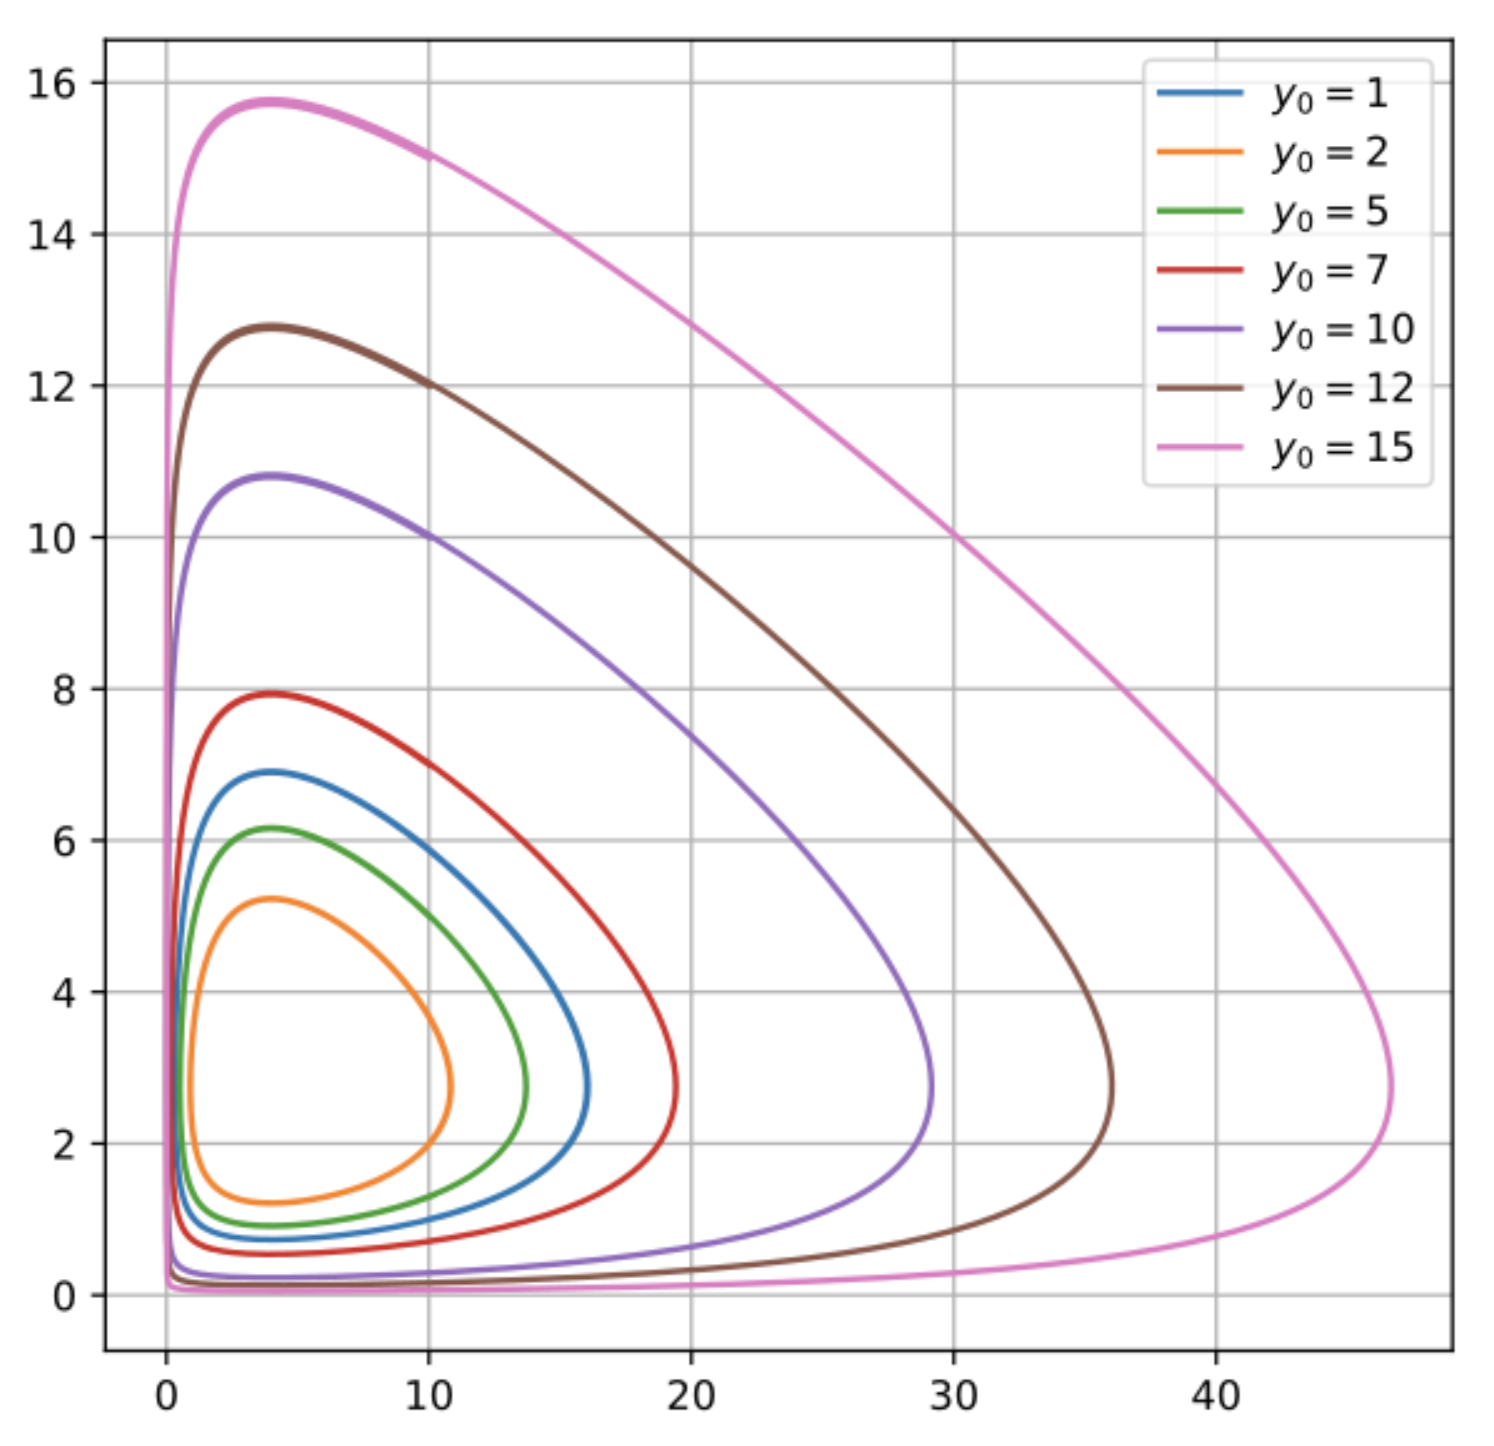
\includegraphics[width=0.4\linewidth]{../ExtFiles/LotkaVolteraSolns.png}
                \caption{Lotka-Volterra solution curves.}
                \label{fig:LotkaVolteraSolns}
            \end{figure}
            \item Properties of the curves:
            \begin{itemize}
                \item The implicit relation which determines them: By the implicit function theorem, the $y$ derivative of the LHS is $B-A/y$ and the $x$-derivative of the LHS is $D-C/x$. When the partial derivatives are equal to zero, $(C/D,A/B)$ becomes interesting. Turning points happen when the $y$-coordinate is $A/B$ or the $x$-coordinate is $C/D$.
            \end{itemize}
        \end{itemize}
    \end{enumerate}
    \item \textbf{Finite lifespan}: Even if the RHS of $\dv*{y}{t}=f(t,y)$ is very regular, the solution can still blow up at some finite time.
    \item Consider the final ODE from the Brachistochrone problem.
    \begin{equation*}
        \dv{y}{x} = \sqrt{\frac{B-y}{y}}
    \end{equation*}
    \begin{itemize}
        \item Finding the \textbf{primitives}.
        \begin{itemize}
            \item What are these "primitives" Shao keeps talking about??
        \end{itemize}
        \item We should have
        \begin{equation*}
            \int\sqrt{\frac{y}{B-y}}\dd{y} = x
        \end{equation*}
        \item Change of variables: $y=B\sin^2\phi$ and $\dd{y}=2B\cos\phi\sin\phi\dd{\phi}$. Thus,
        \begin{equation*}
            \int\sqrt{\frac{y}{B-y}}\dd{y} = \int\frac{\sin\phi}{\cos\phi}\cdot 2B\cos\phi\sin\phi\dd{\phi}
            = 2B\int\sin^2\phi\dd{\phi}
        \end{equation*}
        \item The solution is
        \begin{equation*}
            \begin{cases}
                x = B\phi-\frac{B}{2}\sin(2\phi)+C\\
                y = B\sin^2\phi
            \end{cases}
        \end{equation*}
        \begin{itemize}
            \item This is a parameterization of a cycloid.
        \end{itemize}
    \end{itemize}
    \item Later in the week, we will do the SHM, the pendulum, the Kepler 2-body problem, and the Michaelis-Menten equation.
    \item Separable ODEs are a subset of ODEs of \textbf{exact form}.
    \item ODEs of exact form are of the form
    \begin{equation*}
        g(x,y)\dv{y}{x}+f(x,y) = 0
    \end{equation*}
    where for some $F(x,y)$, $g=\pdv*{F}{y}$, $f=\pdv*{F}{x}$, and partials commute. Equivalently,
    \begin{equation*}
        \pdv{g}{x} = \pdv{f}{y}
    \end{equation*}
    is our necessary and sufficient condition.
    \item By the law of composite differentiation,
    \begin{align*}
        \dv{x}\left[ F(x,y(x)) \right] &= \pdv{F}{x}(x,y(x))+\pdv{F}{y}(x,y(x))\cdot y'(x)\\
        &= f(x,y(x))+g(x,y(x))y'(x)\\
        &= 0
    \end{align*}
    \begin{itemize}
        \item We solve these with an integrating factor $\mu\neq 0$ such that $(\mu g,\mu f)$ satisfy the constraint.
    \end{itemize}
\end{itemize}



\section{Office Hours (Shao)}
\begin{itemize}
    \item \textbf{Primitive}: An antiderivative.
    \item \textbf{Law of composite differentiation}: The chain rule.
    \item Went over how Shao has been applying the law of composite differentiation with respect to separable ODEs:
    \begin{itemize}
        \item Rearrange the initial separable ODE as follows.
        \begin{equation*}
            \frac{1}{g(y)}\cdot\dv{y}{t} = f(t)
        \end{equation*}
        \item Define $\dv*{H}{y}=1/g(y)$. Then, continuing from the above, we have by the law of composite differentiation that
        \begin{align*}
            \dv{H}{y}\cdot\dv{y}{t} &= f(t)\\
            \dv{H}{t} &= f(t)
        \end{align*}
        \item From the definition of $H$, we know that $H(y)=\int_{y_0}^y\dd{w}/g(w)$. We also have from the FTC that $f(t)=\dv{t}\int_{t_0}^tf(\tau)\dd{\tau}$. Thus, continuing from the above, we have that
        \begin{align*}
            \dv{t}(H) &= f(t)\\
            \dv{t}\left[ \int_{y_0}^y\frac{\dd{w}}{g(w)} \right] &= \dv{t}\int_{t_0}^tf(\tau)\dd{\tau}\\
            \dv{t}\left[ \int_{y_0}^{y(t)}\frac{\dd{w}}{g(w)}-\int_{t_0}^tf(\tau)\dd{\tau} \right] &= 0
        \end{align*}
        as desired.
        \item It follows since $y(t_0)=y_0$ that $C=H(y_0)=0$, so we can take the above to
        \begin{equation*}
            \int_{y_0}^{y(t)}\frac{\dd{w}}{g(w)} = \int_{t_0}^tf(\tau)\dd{\tau}
        \end{equation*}
        knowing that our constant of integration is zero.
    \end{itemize}
    \item Take away from Brachistochrone problem: Just an example of a BDE; we won't have to answer questions on it.
\end{itemize}



\section{ODEs of Exact Form}
\begin{itemize}
    \item \marginnote{10/5:}Last time, we discussed separable ODEs.
    \item Today, we will study \textbf{exact form} equations, as discussed last class.
    \item \textbf{Exact form} (ODE): An ODE of the form
    \begin{equation*}
        g(x,y)\dv{y}{x}+f(x,y) = 0
    \end{equation*}
    where
    \begin{equation*}
        \pdv{g}{x} = \pdv{f}{y}
    \end{equation*}
    \item For equations of this form, there exists $F(x,y)$ such that
    \begin{align*}
        \pdv{F}{x} &= f&
        \pdv{F}{y} &= g&
        F(x,y(x)) &= C
    \end{align*}
    for some $C\in\R$.
    \item To solve equations of this form, we need an \textbf{integrating factor}.
    \item \textbf{Integrating factor}: A number or function $\mu$ such that
    \begin{align*}
        \mu g\dv{y}{x}+\mu f &= 0&
        \pdv{x}(\mu g) &= \pdv{y}(\mu f)
    \end{align*}
    \item The solution to linear homogeneous equations of the form $\dv*{y}{t}=p(t)y$ is
    \begin{equation*}
        y(t) = y_0\exp[\int_{t_0}^tp(\tau)\dd\tau]
    \end{equation*}
    \item Recall that $\e[a+ib]=\e[a](\cos b+i\sin b)$, so
    \begin{align*}
        \e[ix] &= \cos x+i\sin x&
        \cos x &= \frac{1}{2}(\e[ix]+\e[-ix])&
        \sin x &= \frac{1}{2i}(\e[ix]-\e[-ix])
    \end{align*}
    \item Example: If $y'=ky$, then $y'=-\lambda y$.
    \item If we have an inhomogeneous linear equation $\dv*{y}{t}=p(t)y+f(t)$, then
    \begin{equation*}
        \dv{y}{t}-py-f = 0
    \end{equation*}
    but
    \begin{equation*}
        0 = \dv{t}(1) \neq \dv{y}(-p(t)y-f(t))
    \end{equation*}
    \item We wish to find an integrating factor $\mu(t,y)$ such that
    \begin{equation*}
        \mu(t,y)\dv{y}{t}-\mu(t,y)p(t)y-\mu(t,y)f(t) = 0
    \end{equation*}
    and
    \begin{equation*}
        \dv{t}(\mu) = \dv{y}(-\mu py-\mu f)
    \end{equation*}
    \item Solution: Take $\mu$ to be a function of $t$, alone. Then
    \begin{equation*}
        \mu'(t) = \dv{y}(-\mu py-\mu f) = -\mu(t)p(t)
    \end{equation*}
    and we now have a homogeneous linear equation with solution
    \begin{equation*}
        \mu(t) = \exp[-\int_{t_0}^tp(\tau)\dd\tau]
    \end{equation*}
    \begin{itemize}
        \item If we let $P(t)=\int_{t_0}^tp(\tau)\dd\tau$, then
        \begin{align*}
            \e[-P(t)]y'(t)-p(t)y(t)\e[-P(t)] &= \e[-P(t)]f(t)\\
            \dv{t}(\e[-P(t)]y(t)) &= \e[-P(t)]f(t)\\
            \e[-P(t)]y(t) &= \int_{t_0}^t\e[-P(\tau)]f(\tau)\dd\tau
        \end{align*}
        \item Thus, we finally have the solution to the inhomogeneous problem as follows: The IVP $y'=py+f$, $y(t_0)=y_0$ has solution
        \begin{equation*}
            y(t) = y_0\e[P(t)-P(t_0)]+\e[P(t)]\int_0^t\e[-P(\tau)]f(\tau)\dd\tau
        \end{equation*}
        where $P$ is any anti-derivative of $p$.
    \end{itemize}
    \item In particular, when $p(t)=a$, we get the \textbf{Duhamel formula} (which we should memorize).
    \item \textbf{Duhamel formula}: The following equation, which is the solution to an inhomogeneous linear equation with $p(t)=a$.
    \begin{equation*}
        y(t) = y_0\e[a(t-t_0)]+\int_{t_0}^t\e[a(t-\tau)]f(\tau)\dd\tau
    \end{equation*}
    \begin{itemize}
        \item Important for computing forced oscillation.
    \end{itemize}
    \item Inspecting the inhomogeneous solution.
    \begin{itemize}
        \item The first term is the solution to the homogeneous form. The second term deals with the initial value.
    \end{itemize}
    \item Given an inhomogeneous equation, you can always write its solution as the combination of the solution to the homogeneous problem plus a particular solution, i.e.,
    \begin{equation*}
        y = y_h+y_p
    \end{equation*}
    \begin{itemize}
        \item "The general solution equals the homogeneous solution plus a particular solution."
        \item This is related to linear algebra, where the solution to $Ax=b$ is a particular solution $x_p$ plus any vector $x\in\ker A$.
        \item Thus, this idea will reappear in the theory of systems of linear ODEs.
    \end{itemize}
    \item We now look at systems of linear ODEs.
    \item Consider the harmonic oscillator: A particle of mass $m$ connected to an ideal spring (obeys Hooke's law) with no friction or gravity.
    \begin{itemize}
        \item Newton's second law: The acceleration is proportional to the restoring force.
        \item Hooke's law: The restoring force is of magnitude $kx$ in the opposite direction to the displacement.
        \item Thus, the ODE is of the form
        \begin{equation*}
            x'' = -\frac{k}{m}x
        \end{equation*}
        \item However, if there is damping (which will be proportional to the velocity), then the ODE is of the form
        \begin{equation*}
            x''+\frac{b}{m}x'+\frac{k}{m}x = 0
        \end{equation*}
    \end{itemize}
    \item Consider an ODE of the form
    \begin{equation*}
        y''+ay'+by = 0
    \end{equation*}
    for $a,b\in\C$.
    \begin{itemize}
        \item Aim: Find $\mu,\lambda\in\C$ such that
        \begin{equation*}
            (y'-\mu y)'-\lambda(y'-\mu y) = 0
        \end{equation*}
        \item To find the parameters, we expand the above to
        \begin{equation*}
            y''-(\mu+\lambda)y'+\mu\lambda y = 0
        \end{equation*}
        \item Comparing with the original form, we have that $a=-(\mu+\lambda)$ and $b=\mu\lambda$.
        \item It follows that $\mu,\lambda$ are the roots of $x^2+ax+b=0$, which we will call the \textbf{characteristic polynomial} of the ODE.
        \item Substitute $x=y'-\mu y$. Then we can solve
        \begin{equation*}
            x'-\lambda x = 0
        \end{equation*}
        to determine that $x=A\e[\lambda t]$.
        \item Returning the substitution, we have that
        \begin{equation*}
            y'-\mu y = A\e[\lambda t]
        \end{equation*}
        \item Since the above is of the form $y'=ay+f$, we can apply the Duhamel formula. It follows that a particular solution is
        \begin{equation*}
            A\int_0^t\e[\mu(t-\tau)]\e[\lambda\tau]\dd\tau
        \end{equation*}
        \item Thus, general solutions are of the form
        \begin{equation*}
            y(t) = B\e[\mu t]+C\e[\mu t]\int_0^t\e[(\lambda-\mu)\tau]\dd\tau
        \end{equation*}
        \item Evaluating the integral, we get
        \begin{equation*}
            y(t) = B\e[\mu t]+C\e[\mu t]\frac{\e[(\lambda-\mu)t]-1}{\lambda-\mu}
        \end{equation*}
        which simplifies (by incorporating constants, etc.) to
        \begin{equation*}
            y(t) = A_1\e[\mu t]+B_1\e[\lambda t]
        \end{equation*}
        for $\mu\neq\lambda$, or
        \begin{equation*}
            y(t) = A_1\e[\mu t]+B_1t\e[\mu t]
        \end{equation*}
        for $\mu=\lambda$.
        \item These linearly independent solutions form a basis of the space of solutions; all solutions can be expressed as a linear combination of these two functions.
    \end{itemize}
    \item If our equation is of the form $y''+ay'+by=f(t)$, then we just need to apply the Duhamel formula twice.
    \item Returning to the simple harmonic oscillator problem, we substitute $\omega=\sqrt{k/m}$ to get
    \begin{equation*}
        x'' = \omega^2x
    \end{equation*}
    \begin{itemize}
        \item The characteristic polynomial is
        \begin{equation*}
            0 = x^2+\omega^2
            = (x+i\omega)(x-i\omega)
        \end{equation*}
        \item Thus, solutions are of the form
        \begin{equation*}
            x = A_1\e[i\omega t]+B_1\e[-i\omega t]
        \end{equation*}
        \item It follows that the period is $T=2\pi/\omega$.
        \item To get a real (usable) solution, apply Euler's formula to get
        \begin{align*}
            x(t) &= A_1(\cos\omega t+i\sin\omega t)+B_1(\cos\omega t-i\sin\omega t)\\
            &= A\cos\omega t+B\sin\omega t
        \end{align*}
        where $A=A_1+B_1$, $B=iA_1-iB_1$.
        \item To match the initial condition $x(0)=x_0$, $x'(0)=v_0$, we use
        \begin{equation*}
            x(t) = x_0\cos\omega t+\frac{v_0}{\omega}\sin\omega t
        \end{equation*}
        \item In other words,
        \begin{align*}
            &
            \begin{cases}
                A=x_0\\
                \omega B=v_0
            \end{cases}
            &&
            \begin{cases}
                A_1+B_1=x_0\\
                i\omega A_1-i\omega B_1=v_0
            \end{cases}
        \end{align*}
        so
        \begin{align*}
            &
            \begin{cases}
                A=x_0\\
                B=\frac{v_0}{\omega}
            \end{cases}
            &&
            \begin{cases}
                A_1=\frac{1}{2}\left[ x_0-\frac{iv_0}{\omega} \right]\\
                B_1=\frac{1}{2}\left[ x_0+\frac{iv_0}{\omega} \right]
            \end{cases}
        \end{align*}
    \end{itemize}
\end{itemize}



\section{ODE Examples}
\begin{itemize}
    \item \marginnote{10/7:}Today, we will investigate a variety of examples of ODEs arising in real life.
    \item Michaelis-Menten kinetics: If E is an enzyme, S is its substrate, and P is the product, then the mechanism is
    \begin{equation*}
        \ce{E + S <=>[$k_1$][$k_{-1}$] ES ->[$k_2$] E + P}
    \end{equation*}
    \item The concentrations that we are concerned with are $\cnc{E},\cnc{S},\cnc{ES},\cnc{P}$.
    \item From the above mechanism, we can write the four rate laws
    \begin{align*}
        \dv{t}\cnc{S} &= -k_1\cnc{E}\cnc{S}+k_{-1}\cnc{ES}\tag{1}\\
        \dv{t}\cnc{E} &= -k_1\cnc{E}\cnc{S}+(k_{-1}+k_2)\cnc{ES}\tag{2}\\
        \dv{t}\cnc{ES} &= k_1\cnc{E}\cnc{S}-(k_{-1}+k_2)\cnc{ES}\tag{3}\\
        \dv{t}\cnc{P} &= k_2\cnc{ES}\tag{4}
    \end{align*}
    \item The initial conditions are $\cnc{S}=\cnc[0]{S}$ and $\cnc{E}=\cnc[0]{E}$.
    \item We can reduce these rate laws to the 2D system
    \begin{align*}
        \dv{t}\cnc{S} &= -k_1(\cnc[0]{E}-\cnc{ES})\cnc{S}+k_{-1}\cnc{ES}\tag{5}\\
        \dv{t}\cnc{ES} &= k_1(\cnc[0]{E}-\cnc{ES})\cnc{S}-(k_{-1}+k_2)\cnc{ES}\tag{6}
    \end{align*}
    \begin{itemize}
        \item Note that to do so, we have used two conservation laws: The conservation of the enzyme plus enzyme-substrate complex, and the conservation of the substrate plus enzyme-substrate complex plus products.
    \end{itemize}
    \item QSSA: Quasi steady-state assumption.
    \begin{itemize}
        \item Assume that $\cnc[0]{E}/\cnc[0]{S}\lll 1$.
        \item It follows that $\dv*{\cnc{ES}}{t}\approx 0$ due to saturation of the enzyme and $\cnc{S}\approx\cnc[0]{S}$ due to ever-more substrate being available.
    \end{itemize}
    \item Then
    \begin{equation*}
        \cnc{ES} = \frac{\cnc[0]{E}\cnc{S}}{K_M+\cnc{S}}
    \end{equation*}
    where $k_M=(k_{-1}+k_2)/k_1$ is the \textbf{Michaelis-Menten constant}, a usual indication of enzyme activity.
    \item Substitute the above into Equation 5:
    \begin{equation*}
        \dv{t}\cnc{S} = -\frac{v_\text{max}\cnc{S}}{k_M+\cnc{S}}
    \end{equation*}
    \begin{itemize}
        \item Note that $v_\text{max}=k_2\cnc[0]{E}$.
    \end{itemize}
    \item The above is now a differential equation of separable form; it's solution is
    \begingroup
    \allowdisplaybreaks
    \begin{align*}
        \int_{\cnc[0]{S}}^{\cnc{S}}-\frac{(k_M+z)\dd{z}}{zv_\text{max}} &= \int_0^t\dd{t}\\
        -\frac{k_M}{v_\text{max}}\log\frac{\cnc{S}}{\cnc[0]{S}}-\frac{1}{v_\text{max}}(\cnc{S}-\cnc[0]{S}) &= t\\
        \log\frac{\cnc{S}}{\cnc[0]{S}}+\frac{\cnc{S}}{k_M} &= \frac{\cnc[0]{S}-v_\text{max}t}{k_M}\\
        \frac{\cnc{S}}{\cnc[0]{S}}\e[\cnc{S}/k_M] &= \exp(\frac{\cnc[0]{S}-v_\text{max}t}{k_M})\\
        \frac{\cnc{S}}{k_M}\e[\cnc{S}/k_M] &= \frac{\cnc[0]{S}}{k_M}\exp(\frac{\cnc[0]{S}-v_\text{max}t}{k_M})\\
        \frac{\cnc{S}}{k_M} &= W\left[ \frac{\cnc[0]{S}}{k_M}\exp(\frac{\cnc[0]{S}-v_\text{max}t}{k_M}) \right]\\
        \cnc{S} &= k_MW\left[ \frac{\cnc[0]{S}}{k_M}\exp(\frac{\cnc[0]{S}-v_\text{max}t}{k_M}) \right]
    \end{align*}
    \endgroup
    \begin{itemize}
        \item Getting from line 5-6 (i.e., the introduction of $W$): Suppose we have an equation of the form $y\e[y]=x$. We cannot express $x$ in terms of $y$ using elementary functions, so we must define $W$ such that $y=W(x)$. Explicitly, $W$ is the unique function of $x$ that satisfies $W(x)\e[W(x)]=x$.
    \end{itemize}
    \item Harmonic oscillator.
    \item Recall that
    \begin{equation*}
        x''+\frac{k}{m}x = 0
    \end{equation*}
    \item Substituting $\omega=\sqrt{k/m}$, we can solve the above for
    \begin{equation*}
        x(t) = x(0)\cos(\omega t)+\frac{x'(0)}{\omega}\sin(\omega t)
    \end{equation*}
    \item This is an integrable system with $n$ degrees of freedom and $n-1$ scalar conservation laws??
    \item Conservation of mechanical energy:
    \begin{equation*}
        E = \frac{1}{2}m|x'|^2+\frac{1}{2}kx^2
    \end{equation*}
    \begin{figure}[h!]
        \centering
        \begin{tikzpicture}
            \footnotesize
            \draw
                (-3,0) -- (3,0) node[right]{$x$}
                (0,-2) -- (0,2) node[above]{$x'$}
            ;

            \draw [rex,thick]
                ellipse (6mm and 4mm)
                ellipse (12mm and 8mm)
                ellipse (18mm and 12mm)
            ;
        \end{tikzpicture}
        \caption{Conservation of mechanical energy in the harmonic oscillator.}
        \label{fig:harmonicEConservation}
    \end{figure}
    \begin{itemize}
        \item Differentiating wrt. $x$ yields
        \begin{align*}
            0 &= mx'x''+kxx'\\
            &= \dv{t}(\frac{1}{2}m(x')^2)+\dv{t}(\frac{1}{2}kx^2)
        \end{align*}
        \item This means that the solution is an ellipse in the $xx'$-plane, where each ellipse corresponds to an initial displacement and velocity.
    \end{itemize}
    \item Mathematical pendulum.
    \item Equation of motion:
    \begin{align*}
        0 &= l\theta''+g\sin\theta\\
        &= \ell\theta''\theta'+g\sin\theta\cdot\theta'\\
        &= \dv{t}\bigg( \underbrace{\frac{\ell}{2}|\theta'|^2-g\cos\theta}_E \bigg)
    \end{align*}
    \item Initial values:
    \begin{align*}
        \theta(0) &= \theta_0&
        \theta'(0) &= 0
    \end{align*}
    \item It follows from the above that
    \begin{align*}
        \frac{\ell}{2}|\theta'|^2-g\cos\theta_0 &= -g\cos\theta\\
        \dv{\theta}{t} &= \sqrt{\frac{2g}{\ell}(\cos\theta_0-\cos\theta)}\\
        \int_{\theta_0}^\theta\sqrt{\frac{\ell}{2g(\cos\theta_0-\cos\phi)}}\dd\phi &= t
    \end{align*}
    \begin{itemize}
        \item This is an elliptical integral (and thus cannot be expressed in terms of the elementary functions).
    \end{itemize}
    \item Suppose $\theta_0$ is small. Then $\theta$ is small, and we can invoke the small angle approximation $\sin\theta\approx\theta$.
    \begin{itemize}
        \item This yields an approximate equation of motion:
        \begin{equation*}
            \ell\theta''+g\theta = 0
        \end{equation*}
        \item From here, we can determine that $\theta(t)\approx\theta_0\cos\sqrt{g/\ell}\cdot t$ and $T=2\pi\sqrt{\ell/g}$.
    \end{itemize}
    \item Kepler problem.
    \item Two bodies of mass $m_1,m_2$ are located at positions $x_1,x_2$ pulling on each other gravitationally.
    \begin{itemize}
        \item The force of attraction is a conservative central force.
        \item The potential between the two masses is a function of their distance, i.e, $U(|x_1-x_2|)$.
    \end{itemize}
    \item From Newton's second and third law, we get
    \begin{align*}
        m_1x_1'' &= U'(|x_1-x_2|)\frac{x_2-x_1}{|x_2-x_1|}&
        m_2x_2'' &= U'(|x_1-x_2|)\frac{x_1-x_2}{|x_1-x_2|}
    \end{align*}
    \begin{itemize}
        \item The derivative of potential is force.
        \item The vector term provides direction.
    \end{itemize}
    \item Conservation of momentum:
    \begin{align*}
        (m_1x_1+m_2x_2)'' &= 0\\
        m_1x_1'+m_2x_2' &= C
    \end{align*}
    \begin{itemize}
        \item Let $M=m_1+m_2$. Then the center of mass
        \begin{equation*}
            \frac{m_1}{M}x_1+\frac{m_2}{M}x_2
        \end{equation*}
        moves inertially (i.e., does not accelerate or decelerate; is a stable reference frame) --- we'll define it to be the origin.
    \end{itemize}
    \item Conservation of angular momentum:
    \begin{equation*}
        [m(x_1-x_2)'\times(x_1-x_2)]' = 0
    \end{equation*}
    \begin{itemize}
        \item $m=m_1m_2/(m_1+m_2)$.
        \item $\times$ indicates the cross product.
        \item $L=m(x_1-x_2)'\times(x_1-x_2)$.
    \end{itemize}
    \item It follows that $x_1-x_2$ is always in a fixed plane, which we may call the \textbf{horizon plane}.
    \item Conservation of mechanical energy:
    \begin{align*}
        mq''+U'(|q|)\frac{q}{|q|} &= 0\\
        \frac{m}{2}|q'|^2+U(|q|) &= E
    \end{align*}
    \begin{itemize}
        \item $q=x_1-x_2$.
    \end{itemize}
    \item Introduce polar coordinates $(r,\phi)$.
    \begin{itemize}
        \item Then $r^2\phi'=\ell_0$, $r=r(\phi)$, and $\dv*{r}{\phi}=r'(t)/\phi'(t)$.
        \item It follows that
        \begin{equation*}
            \frac{m}{2}(|r'|^2+|\phi'|^2)+U(r) = E
        \end{equation*}
        \item Since $U(r)=-Gm_1m_2/r$ for Newtonian gravity,
        \begin{equation*}
            \left( \dv{r}{\phi} \right)^2+r^2 = \frac{2GMr^3}{\ell_0^2}+\frac{2Er^4}{m\ell_0^2}
        \end{equation*}
        \item The substitution $\mu=1/r$ yields
        \begin{equation*}
            \left( \dv{\mu}{\phi} \right)^2+\mu^2 = \frac{2GM}{\ell_0^2}\mu+\frac{2E}{m\ell_0^2}
        \end{equation*}
        \item Differentiating again gives
        \begin{equation*}
            2\dv{\mu}{\phi}\dv[2]{\mu}{\phi}+2\mu\dv{\mu}{\phi} = \frac{2GM}{\ell_0^2}\dv{\mu}{\phi}
        \end{equation*}
        \item Substituting $\mu=\cos(t)$ gives
        \begin{equation*}
            \dv[2]{\mu}{\phi}+\mu-\frac{GM}{\ell_0^2} = 0
        \end{equation*}
        or
        \begin{equation*}
            r = \frac{1}{GM/\ell_0^2+\varepsilon\cos(\phi-\phi_0)}
        \end{equation*}
        \begin{itemize}
            \item This is a conic section!
        \end{itemize}
    \end{itemize}
    \item Thus, for example, we can calculate the precession of Mercury.
    \item Note that while we have determined the trajectory of our 2 bodies in terms of elementary functions, the $n$-body problem cannot be solved analytically.
\end{itemize}



\section{Chapter 1: Introduction}
\emph{From \textcite{bib:Teschl}.}
\subsection*{Section 1.3: First Order Autonomous Equations}
\begin{itemize}
    \item \marginnote{11/15:}We start with the simplest nontrivial case of a first-order autonomous equation:
    \begin{equation*}
        \dot{x} = f(x)
        ,\quad
        x(0) = x_0
    \end{equation*}
    \begin{itemize}
        \item We may let $t_0=0$ WLOG: If $\phi(t)$ is a solution to an autonomous equation satisfying $\phi(0)=x_0$, then $\psi(t)=\phi(t-t_0)$ is a solution with $\psi(t_0)=0$.
    \end{itemize}
    \item Solving this ODE.
    \begin{itemize}
        \item Suppose $f(x_0)\neq 0$. Divide both sides by $f(x)$ and integrate from the initial conditions onward to yield
        \begin{equation*}
            \int_0^t\frac{\dot{x}(s)\dd{s}}{f(x(s))} = t
        \end{equation*}
        \item Define
        \begin{equation*}
            F(x) := \int_{x_0}^x\frac{\dd{y}}{f(y)}
        \end{equation*}
        \begin{itemize}
            \item Note that this is just the previous equation under the "$u$-substitution" $y(t)=x(t)$, $\dd{y}=\dot{x}(t)\dd{t}$, $y(0)=x(0)=x_0$, $y(t)=x$.
        \end{itemize}
        \item Thus, in our new notation, any possible solution $x$ to the ODE must satisfy $F(x(t))=t$. Since $F(x(t))$ is monotone (near $x_0$??), it can thus be inverted to yield the unique solution
        \begin{equation*}
            \phi(t) = F^{-1}(t)
            ,\quad
            \phi(0) = F^{-1}(0) = x_0
        \end{equation*}
    \end{itemize}
    \item \textcite{bib:Teschl} does a deep dive on the maximal integral where $\phi$ is defined.
    \item Examples of first-order autonomous systems given.
    \item Most of this section goes beyond what was covered in class in terms of depth.
\end{itemize}


\subsection*{Section 1.4: Finding Explicit Solutions}
\begin{itemize}
    \item Solving ODEs for explicit solutions is impossible in general unless the equation is of a particular form.
    \item This section: Classes of first-order ODEs which are explicitly solvable.
    \item Strategy: Find a change of variables that transforms the ODE into a solvable form.
    \item Linear equation.
    \begin{align*}
        \dot{x} &= a(t)x&
        \dot{x} &= a(t)x+g(t)
    \end{align*}
    \begin{itemize}
        \item The left equation above is the homogeneous linear equation, and the right equation above is the corresponding inhomogeneous linear equation.
        \item The general solution to the homogeneous linear equation is
        \begin{equation*}
            \phi(t) = x_0A(t,t_0)
        \end{equation*}
        where
        \begin{equation*}
            A(t,s) = \e[\int_s^ta(s)\dd{s}]
        \end{equation*}
        \item The general solution to the inhomogeneous linear equation is
        \begin{equation*}
            \phi(t) = x_0A(t,t_0)+\int_{t_0}^tA(t,s)g(s)\dd{s}
        \end{equation*}
        \item \textcite{bib:Teschl} covers the more detailed mathematics of coordinate transformations in depth. This definitely would have been useful to understand for solving the PSet 1 problems, so I should return and understand it before the final.
    \end{itemize}
    \item Using Mathematica to help solve ODEs and gain an intuition for how they work (e.g., with slope fields).
    \item Equations of exact form are covered in the problems to this section.
\end{itemize}




\end{document}